\documentclass[twoside,11pt]{homework}

\coursename{COMS 4721 Spring 2016}

\studentname{Swapnil Khedekar, Craig Liebman, Felix Matathias}
\studentmail{em2296@columbia.edu,cal2227@columbia.edu,spk2136@columbia.edu}
\usepackage{graphicx}
\begin{document}
\maketitle

\section*{Introduction}

In this brief report we describe the methodology we followed for the in-class Predictive Modeling Competition for COMS 4721, Spring 2016. We developed a binary classifier with an error rate of approximately $5\%$ which performed well in the competition. We chose to completely ignore the domain semantics of the data and our feature selection was solely based on the
characteristics of the input data, including their variance and correlation. In addition to Random Forests, we also tried Logistic Regression, Support Vector Machines, and AdaBoost with Decision Tree as the weak classifier. All classifiers performed relatively well but Random Forest was chosen for its stability and speed. This report is divided in four parts. First we describe the feature selection procedure, then we continue with the comparison of various classifiers, we proceed with the tunning of the winning classifier, and finally we report the results we achieved. 


\section*{Feature Selection}


The feature set is a collection of $52$ numerical and categorical features. We did not conduct any research on the meaning of the feature data but rather conducted a domain agnostic feature selection. In the following we will refer to the columns by their numbers as described in the competition site. We first excluded columns which are linear combinations of other columns. We discovered that columns 18, 23, 25, 26, and, 58 were linear combinations of other columns in the feature set and thus we did not include them in the training process. We then removed columns with no variance, 29, 31, 32, and, 35. Continuing the analysis, columns 38, 39, 40, 41, 42, 43, 44, 45, 46, 47, 48, 49, 50, and, 51, had values in the set $\{1,2,3\}$ and since we did not use any domain knowledge we treated these variables as categorical. The only two real numerical columns, 59, and 60,  were centered and normalized but further analysis proved that they did not have any significant influence in the classification error and thus were dropped too in the final submission in order to produce a simpler model. The pure categorical columns 56, 20, 14, 17, 16, 57, 0, 5, 7, 9, 8, along with the ones we treated as categorical, were converted using a one-hot representation to a final set of 545 feature columns. We further attempted to drop additional numerical columns based on the standard deviation of the data but that did not make any difference in subsequent analysis and we decided to keep them.


The reduction of the initial number of columns had significant impact in the analysis and running time of the algorithms we tested. Without dropping any of the input data, the one-hot representation yielded 5594 columns. After feature selection, the number of columns dropped by an order of magnitude to 545.  


\section*{Algorithm Selection}



We considered three major classes of models in our research: Logistic Regression,
SVM and Random Forests. We started with Logistic Regression for a few reasons.
(1) The algorithm is fast, e.g. compared to SVM.
(2) Even after feature selection, one-hot encoding resulted in 
many features. This initially made us wary of decision trees which if done 
incorrectly can overfit the training data.
(3) At the onset we wanted to establish a baseline classifier and logistic regression is simple in that the model assumes a single linear 
decision boundary. 

Figure 1 contains a plot of C ($1/\lambda$, where $\lambda$ is the regularization term) on the horizontal axis and hold out accuracy on the vertical axis.
It is clear from this plot that for a sufficiently large value of C, meaning the model is not too influenced by regularization,
the classifier plateaus with respect to accuracy. For a baseline this was not too bad but the results pushed us
to consider non-linear models. 

We also experimented with SVM, using both linear and Gaussian (RBF) kernels. We 
focused our effort on the RBF kernel because (1) our available training set had more 
than 100,000 observations and we only had around 500 features after one-hot 
encoding and (2) the results were satisfactory with an error rate slightly below 
our final classifier but the iteration cycle was too long. Some actions we could have 
taken to shrink the iteration cycle are (1) focus on linear kernel and (2) drastically 
shrink the training set.

Figure 1 contains a plot of C (error penalty) on the horizontal axis and hold out accuracy on the vertical axis.
A small value of C tends toward simple decision boundaries while a high value of C (depending on the data) tends toward complicated
decision boundaries. This occurs because C imposes a penalty on misclassifying training samples.
The figure shows that a higher C (at least until C=1000) and more complicated decision boundary actually reflect the overall data
and not just the idiosynchracies of the training samples.

We then turned to ensemble methods. We quickly tried AdaBoost with Decision 
Trees of depth 1 as the weak learner but the results were only slightly better than 
Logistic Regression and definitely worse than SVM. We then turned to Random 
Forests which are ensembles of Decision Trees. What drew us to Random Forests is 
how it uses randomness. Unlike Decision Trees which use all features to make a split 
decision, Random Forests only consider a random subset (of size k, eg 
k=sqrt(number features)) of features at each split decision up to . This gave us the 
power to test different subsets of features, albeit implicitly. From the start Random 
Forest performed on par with SVM, but unlike SVM the runtime is fast and provided 
us with short iteration cycles to tune a few parameters.

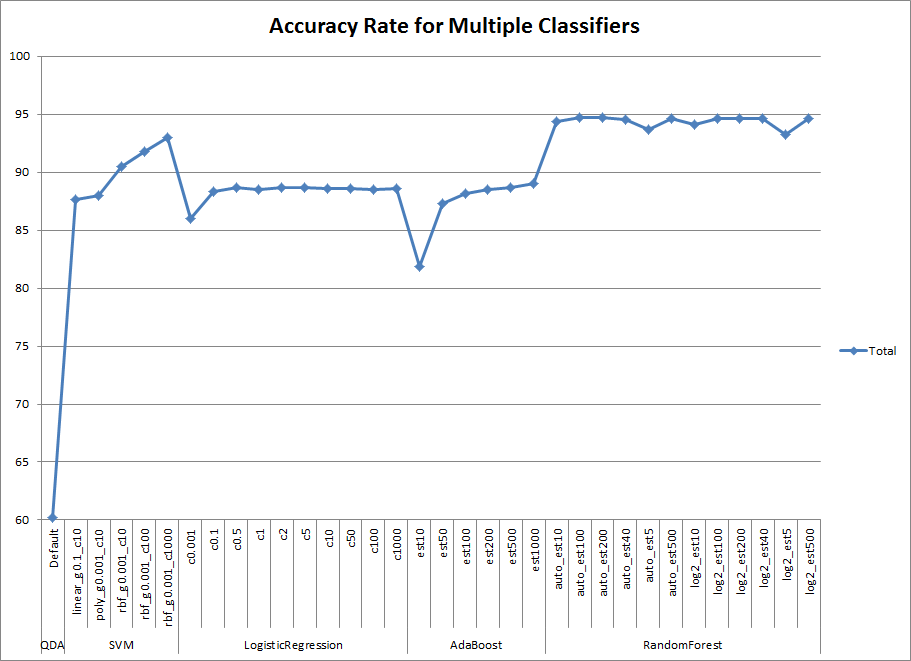
\includegraphics[scale=0.5]{classifiers.png}
Figure 1.

\end{document} 
